% ==============================================================================
% FYDP-I Poster  (A1 portrait, tikzposter)
% "Solving the Lorenz ODE System Using Optimal ANN Architectures"
% United International University - Department of CSE
% Teal theme matched to the institutional reference poster.
% Compile: pdflatex poster.tex
% ==============================================================================
\documentclass[
  14pt,
  a1paper,
  portrait,
  margin=12mm,
  innermargin=11mm,
  blockverticalspace=7mm,
  colspace=12mm,
  subcolspace=8mm
]{tikzposter}

\usepackage{graphicx}
\usepackage{amsmath,amssymb}
\usepackage{booktabs}
\usepackage{array}
\graphicspath{{./figures/}}

% ---------------------------------------------------------------- colours
\definecolor{tealDark}{RGB}{62,124,116}
\definecolor{tealMid}{RGB}{143,196,189}
\definecolor{tealSoft}{RGB}{206,231,228}
\definecolor{ink}{RGB}{32,46,44}
\definecolor{accent}{RGB}{223,150,64}

\usetheme{Default}

\definecolorstyle{LorenzTeal}{
  \definecolor{colorOne}{RGB}{62,124,116}
  \definecolor{colorTwo}{RGB}{143,196,189}
  \definecolor{colorThree}{RGB}{206,231,228}
}{
  \colorlet{backgroundcolor}{white}
  \colorlet{framecolor}{colorOne}
  \colorlet{titlefgcolor}{white}
  \colorlet{titlebgcolor}{colorOne}
  \colorlet{blocktitlebgcolor}{colorTwo}
  \colorlet{blocktitlefgcolor}{ink}
  \colorlet{blockbodybgcolor}{white}
  \colorlet{blockbodyfgcolor}{ink}
  \colorlet{innerblocktitlebgcolor}{colorThree}
  \colorlet{innerblocktitlefgcolor}{ink}
  \colorlet{notebgcolor}{colorThree}
  \colorlet{notefrcolor}{colorOne}
}
\usecolorstyle{LorenzTeal}

\usebackgroundstyle{Empty}
\usetitlestyle{Filled}
\useblockstyle{Default}
\tikzposterlatexaffectionproofoff  % remove the "LaTeX TikZposter" watermark

% ---------------------------------------------------------------- title matter
\title{\parbox{\linewidth}{\centering Solving the Lorenz ODE System\\ Using Optimal ANN Architectures}}
\author{Ikramul Hasan Moral \textbullet\ Md.\ Abu Bakar \textbullet\ Samiur Rahman Omlan \textbullet\ Fariha Islam \textbullet\ Md.\ Touhidul Islam}
\institute{Department of Computer Science and Engineering, United International University \\[3pt]
  \textbf{Team Name:} Team\_ParaDox \quad \textbullet \quad \textbf{Supervisor:} Dr.\ Muhammad Nomani Kabir, Professor, Dept.\ of CSE \quad \textbullet \quad \textbf{Course Teacher:} Dr.\ Md.\ Motaharul Islam, Professor, Dept.\ of CSE}
\titlegraphic{
\includegraphics[width=4.5cm]{uiu.png}}

\begin{document}
\maketitle[width=0.98\linewidth]

\begin{columns}

% =============================================================== LEFT COLUMN
\column{0.5}

\block{Introduction \& Motivation}{
  Coupled nonlinear ODEs like the \textbf{Lorenz-1960} system --- an early meteorological
  model of three coupled equations --- rarely have closed-form solutions. Classical solvers
  (Runge--Kutta) are accurate but \textbf{mesh-dependent} and re-solve step-by-step for every
  query. A trained network can instead learn the continuous map $t\mapsto(x,y,z)$, yet most
  neural ODE work relies on physics-informed losses or operator learning.
  \vspace{2mm}

  \innerblock{Central question}{
    Can a \textbf{plain feedforward ANN} --- trained only on numerical data, no physics in the
    loss --- approximate the Lorenz-1960 solution, and \emph{which architecture does it best}?
  }
}

\block{Objectives}{
  \begin{itemize}
    \item Generate a trusted reference with RK4 \emph{and} SciPy; cross-validate the two.
    \item Systematically vary \textbf{depth}, \textbf{width}, and \textbf{activation} (plain ANN).
    \item Evaluate accuracy vs.\ cost: MSE, MAE, max error, training/inference time.
    \item Benchmark the best plain ANN against PINN / DeepONet results.
  \end{itemize}
}

\block{Research Questions \& Gap}{
  \textbf{Gap.} No prior work runs a systematic plain-ANN architecture study on Lorenz-1960;
  existing studies fix the architecture, use only simple ODEs, or rely on physics-informed losses.
  \begin{itemize}
    \item Can a plain ANN learn the solution from numerical data alone?
    \item Which depth $\times$ width $\times$ activation gives the best accuracy--cost trade-off?
    \item How close does it come to physics-informed baselines?
  \end{itemize}
}

\block{Background: System \& Network}{
  \begin{minipage}[c]{0.46\linewidth}
    Three coupled nonlinear ODEs; with $k=2,\ l=1$:
    \[
    \begin{aligned}
      \dot{x}&=kl\!\left(\tfrac{1}{k^2+l^2}-\tfrac{1}{k^2}\right)yz\\[2pt]
      \dot{y}&=kl\!\left(\tfrac{1}{l^2}-\tfrac{1}{k^2+l^2}\right)xz\\[2pt]
      \dot{z}&=\tfrac{kl^2}{2}\!\left(\tfrac{1}{k^2}-\tfrac{1}{l^2}\right)xy
    \end{aligned}
    \]
    {\small $x_0{=}0.5,\ y_0{=}0.75,\ z_0{=}1,\ t\in[0,1]$.}
  \end{minipage}\hfill
  \begin{minipage}[c]{0.50\linewidth}
    \centering
    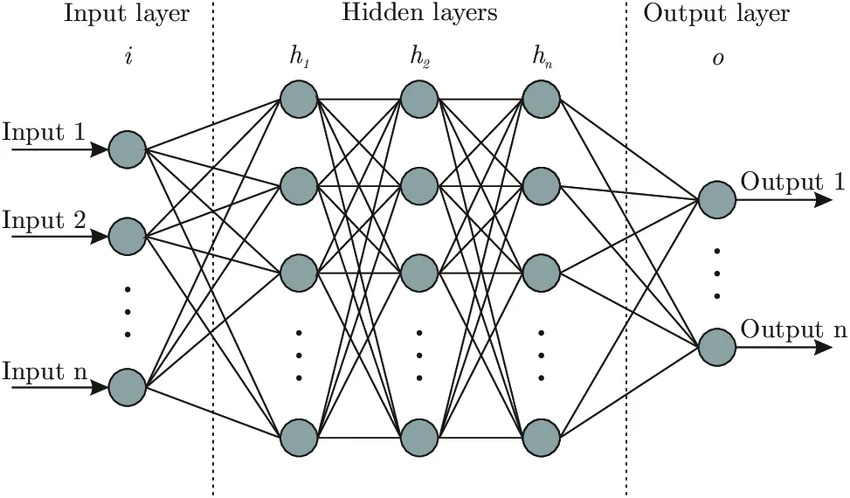
\includegraphics[width=\linewidth]{ann_architecture.jpg}\\[2pt]
    {\small Plain ANN: learns $t\mapsto(x,y,z)$ by backpropagation. PINNs are used only as a literature benchmark.}
  \end{minipage}
}

\block{Complex Engineering Problem}{
  Mapped to the CEP rubric --- \textbf{problem solving} (depth of knowledge, conflicting
  requirements, depth of analysis, interdependence), \textbf{activities} (resources, interaction,
  innovation, unfamiliarity), and \textbf{knowledge} (natural sciences, mathematics, engineering
  fundamentals, specialist ML, research literature, ethics).
}

% =============================================================== RIGHT COLUMN
\column{0.5}

\block{Methodology: Two-Phase Study}{
  \begin{minipage}[t]{0.52\linewidth}
    \innerblock{Phase 1 --- Architecture search}{
      depth $\{1,2,3,4\}$ $\times$ width $\{20,50,100\}$ $\times$
      activation $\{$tanh, ReLU, sigmoid, GELU, Swish$\}$
      \\[2pt]\centering\textbf{= 60 runs} (Adam fixed)
    }
    \vspace{2mm}
    \innerblock{Phase 2 --- Optimizers}{
      3 best architectures $\times$ \{Adam, L-BFGS, SGD+momentum\}
      \\[2pt]\centering\textbf{= 9 runs}
    }
    \vspace{2mm}
    \centering\textbf{69 controlled experiments} --- this split cleanly separates architecture
    effects from optimizer effects.
  \end{minipage}\hfill
  \begin{minipage}[t]{0.44\linewidth}
    \centering
    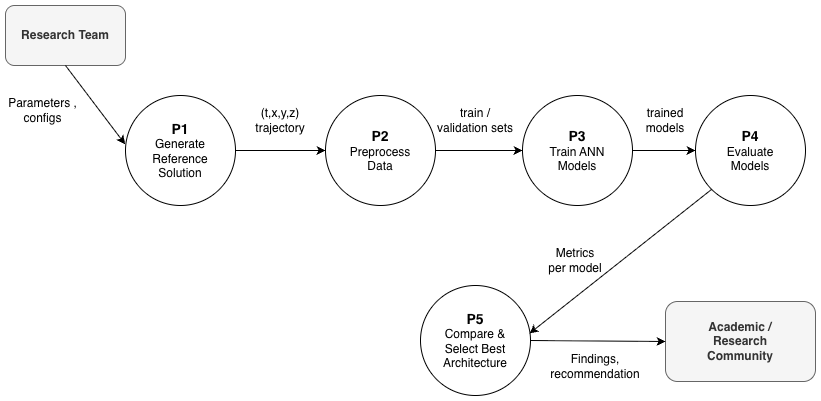
\includegraphics[width=\linewidth]{dfd_level1.png}\\[2pt]
    {\small Pipeline: generate $\to$ preprocess $\to$ train $\to$ evaluate $\to$ select.}
  \end{minipage}
}

\block{Numerical Baseline \& Validation (Result)}{
  The reference trajectory is generated by two independent solvers and cross-checked before any
  ANN sees it: a custom \textbf{RK4} integrator ($h{=}10^{-3}$, 1001 points) and \textbf{SciPy
  DOP853} ($\text{rtol}{=}10^{-10}$), with an 80/20 train/validation split (seed 42).
  \vspace{2mm}

  \centering
  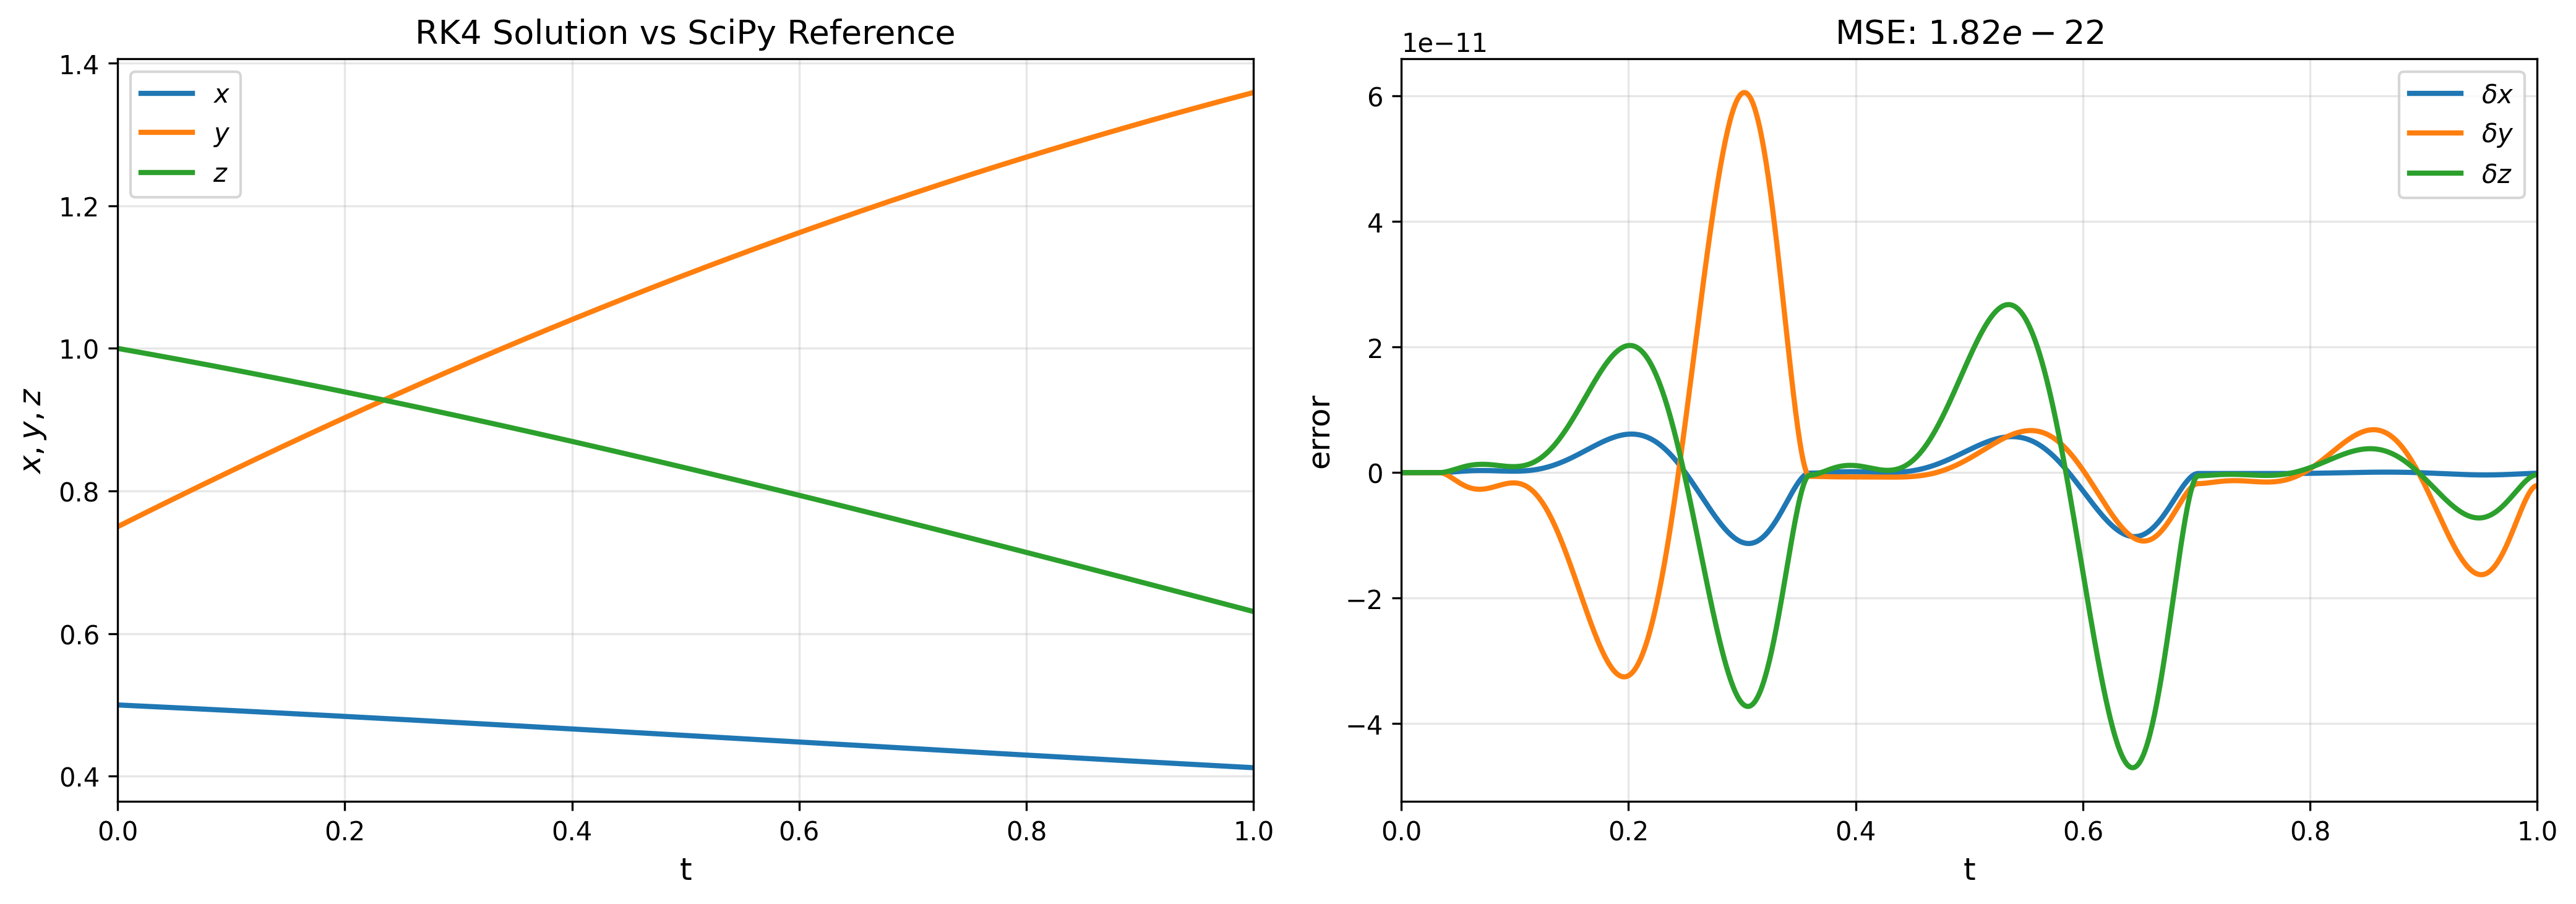
\includegraphics[width=0.98\linewidth]{lorenz1960_comparison.png}\\[2pt]
  \raggedright
  The two solvers agree to \textbf{MSE $\approx 1.8\times10^{-22}$}, far below the $10^{-10}$
  target --- a defensible \textbf{ground truth} for all FYDP-II ANN training.
}

\block{Conclusion \& Future Work}{
  \textbf{Status (FYDP-I):} research question framed, 17-paper review with an explicit gap,
  two-phase design (69 runs) locked, dual-solver baseline verified. No accuracy claims are made
  until the FYDP-II experiments produce evidence.
  \begin{itemize}
    \item Build the ANN training pipeline; run Phase 1 (60), then Phase 2 (9).
    \item Repeated seeds for stability; denser grids and new initial conditions.
    \item Direct comparison with PINN / operator-learning baselines.
  \end{itemize}
}

\block{Selected References}{
  \small
  [1] Lorenz (1960), \textit{Tellus} 12(3). \quad [2] Matthews \& Bihlo (2024), PinnDE.\par
  [3] Raissi et al.\ (2019), \textit{J.\ Comput.\ Phys.}\ 378. \quad [4] Lagaris et al.\ (1998), \textit{IEEE TNN} 9(5).\par
  [5] Lau \& Werth (2020), ODEN. \quad [6] Mall \& Chakraverty (2013). \quad [7] Chen et al.\ (2018), Neural ODEs.
}

\end{columns}

\end{document}
